%%%%%%%%%%%%%%%%%%%%%%%%%%%%%%%%%%%%%%%%%%%%%%%%%%%%%%%%%%%%%%%%%%%%%%%%%%%%%
%%% LaTeX-Rahmen fuer das Erstellen von Diplomarbeiten
%%%%%%%%%%%%%%%%%%%%%%%%%%%%%%%%%%%%%%%%%%%%%%%%%%%%%%%%%%%%%%%%%%%%%%%%%%%%%

%%%%%%%%%%%%%%%%%%%%%%%%%%%%%%%%%%%%%%%%%%%%%%%%%%%%%%%%%%%%%%%%%%%%%%%%%%%%%
%%% allgemeine Einstellungen
%%%%%%%%%%%%%%%%%%%%%%%%%%%%%%%%%%%%%%%%%%%%%%%%%%%%%%%%%%%%%%%%%%%%%%%%%%%%%

\documentclass[twoside,12pt,a4paper]{report}
%\usepackage{reportpage}
\usepackage[utf8]{inputenc}
\usepackage{epsf,german}
\usepackage{graphics, graphicx}
\usepackage{latexsym}
\usepackage{amsfonts}
\usepackage{amsmath}
\usepackage{listings}
\usepackage{url}
\usepackage{textcomp}
\usepackage[numbers]{natbib}
\usepackage[margin=10pt,font=small,labelfont=bf]{caption}
\usepackage{xcolor}
\usepackage{hyperref}
\definecolor{darkred}{rgb}{0.5,0,0}
\definecolor{red}{rgb}{1,0,0}
\definecolor{darkgreen}{rgb}{0,0.5,0}
\definecolor{darkblue}{rgb}{0,0,0.5}
\definecolor{gray}{gray}{.6}

\definecolor{javared}{rgb}{0.6,0,0} % for strings
\definecolor{javagreen}{rgb}{0.25,0.5,0.35} % comments
\definecolor{javapurple}{rgb}{0.5,0,0.35} % keywords
\definecolor{javadocblue}{rgb}{0.25,0.35,0.75} % javadoc


%\lstloadlanguages{Java,XML,HTML,C++,SQL,C}
\hypersetup{colorlinks,
linkcolor=darkblue,
citecolor=darkgreen,
urlcolor=blue
}

\lstdefinelanguage[Objective]{C}[GNU99]{C}
  {morekeywords={@catch,@class,@encode,@end,@finally,@implementation,%
      @interface,@private,@protected,@protocol,@public,@selector,%
      @synchronized,@throw,@try,BOOL,Class,IMP,NO,Nil,SEL,YES,_cmd,%
      bycopy,byref,id,in,inout,nil,oneway,out,self,super,%
      % The next two lines are Objective-C 2 keywords.
      @dynamic,@package,@property,@synthesize,readwrite,readonly,%
      assign,retain,copy,nonatomic%
      },%
   moredirectives={import}%
  }%

\lstdefinelanguage[GNU99]{C}[99]{C}
  {morekeywords={asm,__asm__,__extension__,typeof,__typeof__}%
  }%

\lstdefinelanguage[99]{C}%
  {morekeywords={_Bool,_Complex,_Imaginary,auto,break,case,char,%
      const,continue,default,do,double,else,enum,extern,float,for,%
      goto,if,inline,int,long,register,restrict,return,short,signed,%
      sizeof,static,struct,switch,typedef,union,unsigned,void,volatile,%
      while},%
   sensitive,%
   morecomment=[s]{/*}{*/},%
   morecomment=[l]//,%
   morestring=[b]",%
   morestring=[b]',%
   moredelim=*[directive]\#,%
   moredirectives={define,elif,else,endif,error,if,ifdef,ifndef,line,%
      include,pragma,undef,warning}%
  }[keywords,comments,strings,directives]%

\lstset{language=[Objective]C, 
	breakindent=40pt, 
	breaklines, 
	basicstyle=\ttfamily\color{black}\scriptsize,
	keywordstyle=\color{javapurple}\bfseries,
	stringstyle=\color{javared},
	commentstyle=\color{javagreen},
	morecomment=[s][\color{javadocblue}]{/**}{*/},
	numbers=right,
	numberstyle=\tiny\color{black},
	stepnumber=1,
	numbersep=10pt,
	tabsize=2,
	showspaces=false,
	showstringspaces=false,
	frame=single,
	escapeinside={(*@}{@*)},
	title=\lstname,
	captionpos=b,
}




\textwidth 14cm
\textheight 22cm
\topmargin 0.0cm
\evensidemargin 1cm
\oddsidemargin 1cm
%\footskip 2cm
\parskip0.5explus0.1exminus0.1ex

% Kann von Student auch nach persönlichem Geschmack verändert werden.
\pagestyle{headings}

\sloppy

\begin{document}
\setlength\parindent{0pt} 


%%%%%%%%%%%%%%%%%%%%%%%%%%%%%%%%%%%%%%%%%%%%%%%%%%%%%%%%%%%%%%%%%%%%%%%%%%%%
%%% hier steht die neue Titelseite 
%%%%%%%%%%%%%%%%%%%%%%%%%%%%%%%%%%%%%%%%%%%%%%%%%%%%%%%%%%%%%%%%%%%%%%%%%%%%
 
\begin{titlepage}
	\begin{center}
  		{\LARGE Eberhard Karls Universität Tübingen}\\
		{\large Mathematisch-Naturwissenschaftliche Fakultät \\
		Wilhelm-Schickard-Institut für Informatik\\[4cm]}
  		{\huge Studienarbeit Informatik\\[2cm]}
  		{\Large\bf  Orientierungsberechnung mittels Multisensordatenfusion auf iOS-Endgeräten\\[1.5cm]}
 		{\large Sebastian Engel}\\[0.5cm]
		26.02.2012 \\[4cm]
		{\small\bf Betreuer}\\[0.5cm]
  		\parbox{7cm}{
  			\begin{center}
				{\large Jürgen Sommer}\\
	  			{\footnotesize Wilhelm-Schickard-Institut für Informatik\\
				Universität Tübingen}
			\end{center}
 		}
 	\end{center}
\end{titlepage}

%%%%%%%%%%%%%%%%%%%%%%%%%%%%%%%%%%%%%%%%%%%%%%%%%%%%%%%%%%%%%%%%%%%%%%%%%%%%
%%% Titelrückseite: Bibliographische Angaben
%%%%%%%%%%%%%%%%%%%%%%%%%%%%%%%%%%%%%%%%%%%%%%%%%%%%%%%%%%%%%%%%%%%%%%%%%%%%

\thispagestyle{empty}
\vspace*{\fill}
\begin{minipage}{11.2cm}
\textbf{Engel, Sebastian:}\\
\emph{Orientierung von Objekten bei inertialer Navigation}\\ Studienarbeit Informatik\\
Eberhard Karls Universität Tübingen\\
Bearbeitungszeitraum: 10/2011 - 01/2012
\end{minipage}
\newpage

%%%%%%%%%%%%%%%%%%%%%%%%%%%%%%%%%%%%%%%%%%%%%%%%%%%%%%%%%%%%%%%%%%%%%%%%%%%%

\pagenumbering{roman}
\setcounter{page}{1}

%%%%%%%%%%%%%%%%%%%%%%%%%%%%%%%%%%%%%%%%%%%%%%%%%%%%%%%%%%%%%%%%%%%%%%%%%%%%
%%% Seite I: Zusammenfassug, Danksagung
%%%%%%%%%%%%%%%%%%%%%%%%%%%%%%%%%%%%%%%%%%%%%%%%%%%%%%%%%%%%%%%%%%%%%%%%%%%%


\section*{Zusammenfassung}

Im Rahmen eines Navigations-Programms für Bibliotheken auf mobilen Geräten der neusten Generation beschäftigt sich diese Studienarbeit mit der Orientierung (Winkellage) des Geräts. Zur genauen Navigation in Räumen genügt die Bestimmung der Position nicht. Es ist zusätzlich relevant wie das Gerät orientiert ist. Durch diese Information ist es möglich, den Benutzer direkt zu einem bestimmten Ort, im Falle einer Bibliothek ein Buch, zu führen. Im Wesentlichen befasst sich die Studienarbeit mit der Beschaffung und Berechnung der Orientierungsdaten.

\newpage
\section*{Danksagung}

Vielen Dank an Jürgen Sommer, Alex Decker, Achim Fritz, Stephan Doerr, Martin Lahl, Philipp Wolter, Markus ... und Sabrina Pfeffer.

\cleardoublepage

%%%%%%%%%%%%%%%%%%%%%%%%%%%%%%%%%%%%%%%%%%%%%%%%%%%%%%%%%%%%%%%%%%%%%%%%%%%%%
%%% Inhaltsverzeichnis
%%%%%%%%%%%%%%%%%%%%%%%%%%%%%%%%%%%%%%%%%%%%%%%%%%%%%%%%%%%%%%%%%%%%%%%%%%%%%

\renewcommand{\baselinestretch}{1.3}
\small\normalsize

\tableofcontents

\renewcommand{\baselinestretch}{1}
\small\normalsize

\cleardoublepage

%%%%%%%%%%%%%%%%%%%%%%%%%%%%%%%%%%%%%%%%%%%%%%%%%%%%%%%%%%%%%%%%%%%%%%%%%%%%%
%%% Abbildungsverzeichnis
%%%%%%%%%%%%%%%%%%%%%%%%%%%%%%%%%%%%%%%%%%%%%%%%%%%%%%%%%%%%%%%%%%%%%%%%%%%%%

\renewcommand{\baselinestretch}{1.3}
\small\normalsize

\addcontentsline{toc}{chapter}{Abbildungsverzeichnis}
\listoffigures

\renewcommand{\baselinestretch}{1}
\small\normalsize

\cleardoublepage

%%%%%%%%%%%%%%%%%%%%%%%%%%%%%%%%%%%%%%%%%%%%%%%%%%%%%%%%%%%%%%%%%%%%%%%%%%%%%
%%% Listingverzeichnis
%%%%%%%%%%%%%%%%%%%%%%%%%%%%%%%%%%%%%%%%%%%%%%%%%%%%%%%%%%%%%%%%%%%%%%%%%%%%%

\renewcommand{\baselinestretch}{1.3}
\small\normalsize

\addcontentsline{toc}{chapter}{Listingverzeichnis}
\lstlistoflistings

\renewcommand{\baselinestretch}{1}
\small\normalsize

\cleardoublepage

%%%%%%%%%%%%%%%%%%%%%%%%%%%%%%%%%%%%%%%%%%%%%%%%%%%%%%%%%%%%%%%%%%%%%%%%%%%%%
%%% Abkürzungsverzeichnis
%%%%%%%%%%%%%%%%%%%%%%%%%%%%%%%%%%%%%%%%%%%%%%%%%%%%%%%%%%%%%%%%%%%%%%%%%%%%%

\addcontentsline{toc}{chapter}{Abkürzungsverzeichnis}
\chapter*{Abkürzungsverzeichnis\markboth{ABKÜRZUNGSVERZEICHNIS}{ABKÜRZUNGSVERZEICHNIS}}

\begin{tabbing}
\textbf{FACTOTUM}\hspace{1cm}\=Schrott\kill
\textbf{IMU}\>Inertial Measuring Unit \\
\textbf{API} \> Application Programming Interface\\
\textbf{GPS} \> Global Positioning System\\
\textbf{MEMS} \> Microelectromechanical Systems\\
\textbf{RSSI} \> Received Signal Strength Indication\\
\textbf{NFC} \> Near Field Communication\\
\textbf{RFID} \> Radio-Frequency Identification\\
\end{tabbing}

\cleardoublepage

%%%%%%%%%%%%%%%%%%%%%%%%%%%%%%%%%%%%%%%%%%%%%%%%%%%%%%%%%%%%%%%%%%%%%%%%%%%%%
%%% Der Haupttext, ab hier mit arabischer Numerierung
%%% Mit \input{dateiname} werden die Datei `dateiname' eingebunden
%%%%%%%%%%%%%%%%%%%%%%%%%%%%%%%%%%%%%%%%%%%%%%%%%%%%%%%%%%%%%%%%%%%%%%%%%%%%%

\pagenumbering{arabic}
\setcounter{page}{1}

%% Introduction
%%%%%%%%%%%%%%%%%%%%%%%%%%%%%%%%%%%%%%%%%%%%%%%%%%%%%%%%%%%%%%%%%%%%
% Einleitung
%%%%%%%%%%%%%%%%%%%%%%%%%%%%%%%%%%%%%%%%%%%%%%%%%%%%%%%%%%%%%%%%%%%%

\chapter{Einleitung}\label{Einleitung}

\medskip
Die Arbeit gliedert sich wie folgt: Zu Beginn wird in Kapitel~\ref{Stand der Technik} die Entwicklung der benötigten Hard- und Software betrachtet. In Kapitel~\ref{Konzept} wird ein Konzept zur Berechnung der Orientierung eines mobilen Geräts entwickelt. Bevor sich der genauen Implementierung, am Beispiel einer Navigations-App für Bibliotheken, in Kapitel~\ref{Umsetzung} gewidmet wird, werden in Kapitel~\ref{Plattform und Werkzeuge} die für diese Herangehensweise geeignete Plattform und Werzkeuge gewählt, die zur Umsetzung benötigt werden. Die Umsetzung erfolgt auf Basis der eingebauten Sensoren. Es soll keine Zusatzhardware zum Einsatz kommen. Es folgt eine Auswertung der Ergebnisse in Kapitel~\ref{Ergebnis} mit einer Diskussion. Am Ende beschließt ein Ausblick in Kapitel~\ref{Ausblick} diese Arbeit. Die Studienarbeit entwickelt eine Diplomarbeit von Achim Fritz aus dem Jahr 2011 weiter.

\section{Motivation}\label{Motivation}
Bisher findet Navigation hauptsächlich im Freien statt – beispielsweise schon seit Langem bei Navigationssystemen für Autos. Dabei wird ausschließlich GPS verwendet. Für Navigation innerhalb von Gebäuden ist GPS aber nicht brauchbar. Es ist zu ungenau und wird durch die Wände des Gebäudes noch zusätzlich ungenauer. Bei der genauen Positionsbestimmung wird es zunehmend wichtiger, auch die Orientierung zu bestimmen. Denn innerhalb von Gebäuden und bei Positionsunterschieden von wenigen Metern ist die Information, in welche Richtung man schaut, ebenfalls interessant und liefert zusätzliche Informationen. Gerade bei einer Navigations-App für Bibliotheken ist es wichtig zu wissen, welches Regal im Moment angeschaut wird. Außerdem darf die Position eine Ungenauigkeit von einigen Zentimetern nicht überschreiten. Ziel dieser Arbeit ist es die Lage des Geräts im Raum zu berechnen. Die aus den Werten der Sensoren des Geräts berechneten Werte sollen für eine bereits bestehende praxistaugliche Navigations-App für Bibliotheken die Orientierungs-Werte beisteuern.
\cleardoublepage

%% 
%%%%%%%%%%%%%%%%%%%%%%%%%%%%%%%%%%%%%%%%%%%%%%%%%%%%%%%%%%%%%%%%%%%%
% Grundlagen
%%%%%%%%%%%%%%%%%%%%%%%%%%%%%%%%%%%%%%%%%%%%%%%%%%%%%%%%%%%%%%%%%%%%

\chapter{Stand der Technik}
  \label{Stand der Technik}

\medskip
Bisher findet Navigation hauptsächlich im Freien statt. Zum Beispiel schon seit Langem bei Navigationssystemen für Autos. Dabei wird ausschließlich GPS verwendet. Für Navigation innerhalb von Gebäuden ist GPS nicht brauchbar. Es ist zu ungenau und wird durch die Wände des Gebäudes noch zusätzlich ungenauer. Bei der genauen Positionsbestimmung wird es zunehmend wichtiger, auch die Orientierung zu bestimmen. Denn innerhalb von Gebäuden und bei Positionsunterschieden von wenigen Metern ist die Information, in welche Richtung man schaut, ebenfalls interessant und liefert zusätzliche Informationen. Gerade bei einer Navigations-App für Bibliotheken ist es wichtig zu wissen, welches Regal im Moment angeschaut wird. Außerdem darf die Position eine Ungenauigkeit von einigen Zentimetern nicht überschreiten.

\section{Beschreibung der Orientierung von Objekten im dreidimensionalen Raum}
Zur Beschreibung der Orientierung von Objekten im dreidimensionalen Raum in kartesischen Koordinatensystemen gibt es mehrere Möglichkeiten. Die drei am häufigsten verwendeten und für uns relevanten werden im Folgenden vorgestellt.

\subsection{Euler-Winkel}
Bei Euler-Winkeln handelt es sich um drei Winkel, die jeweils die Rotation um eine bestimmte Achse des Koordinatensystems angeben. So kann eine Transformation zwischen zwei Koordinatensystemen, dem Labor- und dem Körperfesten-System definiert werden.

Es existieren mehrere Definitionen von Euler-Winkeln, was die Reihenfolge der Drehungen um die Achsen anbelangt. Für unsere Zwecke beschäftigen wir uns mit Yaw-Pitch-Roll - zu deutsch: Roll-Nick-Gier-Winkel. Dies entspricht auch der Luftfahrtnorm (DIN 9300).

\begin{itemize}
	\item Roll (Roll-Winkel) beschreibt die Querneigung, also die Drehung um die X-Achse.
	\item Pitch (Nick-Winkel) besschreibt die Längsneigung, also die Drehung um die Y-Achse.
	\item Yaw (Gier-Winkel) beschreibt Orientierung, also die Drehung um die Z-Achse.
\end{itemize}

Bei mobilen Geräten wie dem Apple iPhone, gibt es anders als bei Fahrzeugen, keine fest definierte Ausrichtung. Beim iPhone und iPad sind die Winkel darum so verteilt wie auf Abbildung \ref{fig:apple-axes} zu sehen.

\begin{figure}[htb]
\centering
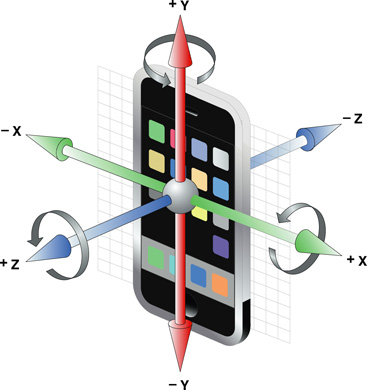
\includegraphics[scale=0.8]{figures/apple-axes}
\caption{Roll-Pitch-Yaw \cite{apple:001}}
\label{fig:apple-axes}
\end{figure}

Euler-Winkel haben den Vorteil, dass sie jeder intuitiv verstehen kann. Jeder lernt Euler-Winkel in der Schule kennen. Somit kann man mit ihnen auch einfach rechnen.

Eine Drehung mit Euler-Winkeln setzt sich immer aus einer Kombination von Rotation der drei Achsen zusammen. Das heißt, eine Drehung findet nie direkt statt, sondern über mehrere nacheinander ausgeführte Rotationen der einzelnen Achsen. Das kann bei manchen Anwendungen ein Problem sein. Zum Beispiel wenn die Orientierung schneller abgefragt wird als die Teilschritte einer Drehung berechnet werden, kann es vorkommen, dass in einzelnen Key-Frames der Anwendung falsche Orientierungsdaten einfließen.

Eine Orientierungs-Angabe als Euler-Winkel würde beispielsweise wie folgt aussehen: 
$$
\begin{pmatrix}
    0.016134\\ 
    -0.000284\\ 
    1.618407
  \end{pmatrix} 
$$
Die Werte sind in Radiant angeben. Negative Werte können zustande kommen, da die Skala von $-\pi$ bis $+\pi$ geht.

\subsubsection{Gimbal Lock}
Der große Nachteil von Euler-Winkeln ist der Gimbal Lock (engl. f. Blockade der Kardanischen Aufhängung). So nennt man es wenn zwei Achsen die selbe Drehung bestimmen. Dadurch fehlt ein Freiheitsgrad. Man kann eine bestimmte Drehung erst dann wieder durchführen, wenn man eine der beiden zusammengefallenen Achsen zurück dreht. In Abbildung \ref{fig:gimbal-lock} ist leicht zu erkennen, dass die innere (blau) und äußere (grün) Achse die selbe Drehung bestimmen. Es ist daher momentan nicht möglich, das Flugzeug nach vorne oder hinten zu kippen. Zuerst müsste das Flugzeug entlang der mittleren Achse um $90^o$ gedreht werden. \cite{ wiki:002} \cite{paper:001}

\begin{figure}[htb]
\centering
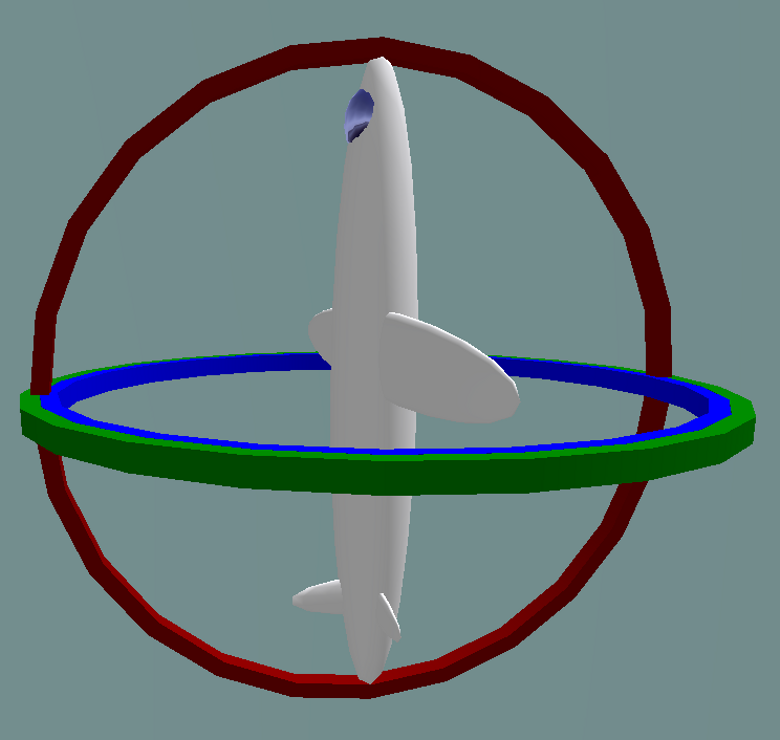
\includegraphics[scale=0.4]{figures/gimbal-lock}
\caption{Gimbal Lock \cite{ wiki:004} }
\label{fig:gimbal-lock}
\end{figure}

\subsection{Rotationsmatrizen}
Eine Rotationsmatrix ist eine orthogonale Matrix, die ebenfalls die Drehung im Raum beschreibt. Sie ist als eine Hintereinanderausführung einer oder mehrerer Rotationen um beliebige Drehachsen im dreidimensionalen Raum definiert. Rotationsmatrizen sind also eine Zusammenfassung von einzelnen Rotationen mit Euler-Winkeln in ein einziges Konstrukt. Gimbal Lock kann auch mit Rotationsmatrizen auftreten. \cite{ wiki:003}

\subsection{Quaternionen}
Quaternionen sind ein mathematisches Konstrukt, um Orientierung von Objekten im dreidimensionalen Raum zu beschreiben. Sie setzen sich aus einem skalaren und einem vektoriellen Teil zusammen. Der vektorielle Teil ist allein dazu da, um die Achse der durchzuführenden Drehung zu beschreiben. Der Skalaranteil gibt den Winkel der Drehung an. Es wird also für jede Rotation eine eigene Achse konstruiert entlang der gedreht wird. Dadurch gibt es keine Zwischenschritte, sondern nur eine einzige Rotation. So kann auch das Problem des Gimbal Locks garnicht erst entstehen.

\section{Positionsbestimmung}
Die Positionsbestimmung erfolgt in unserem Fall über Bluetooth. Dazu werden in dem Raum, in dem man navigieren möchte, Bluetooth-Sender (Beacons) ausgelegt. Diese sollten möglichst gleichmäßig verteilt sein, damit eine gleichmäßige Bluetooth-Abdeckung gewährleistet ist. Die App weiß, wo sich die einzelnen Beacons im Raum befinden und empfängt die RSSI-Werte der ausgelegten Beacons und kann so die Position des Geräts bestimmen. 

Dabei können mehrere Probleme auftreten. Das größte ist die Senderate der Beacons. Herkömmliche Bluetooth-Sticks sind dafür gemacht, eine ständige Verbindung zu einem Gerät aufrechtzuerhalten um Daten zu übertragen. Bei unserem Anwendungsfall wollen wir keine Daten übertragen, sondern nur möglichst oft den RSSI-Wert der einzelnen Beacons erfahren. Normale Bluetooth-Sticks schaffen meistens nur eine Rate von ca. drei Sekunden. Das ist zu wenig um mit wenigen Sticks eine zuverlässige Navigation zu realisieren. Man muss entweder in relativ teure (über 100\texteuro) Bluetooth-Sender investieren die schnell sind, oder viele von den langsameren Sendern auslegen.

Ein weiteres Problem ist, dass Bluetooth leicht gestört werden kann. Personen, Wände und Bücherregale sind ein Problem bei Bluetooth. Darum kann man nicht sicher sein, dass die RSSI-Werte, die beim Gerät ankommen, die entsprechende Entfernung repräsentieren. 

Um diesen beiden Hauptproblemen entgegenzuwirken, wird ein Partikelfilter eingesetzt. Mit dem Partikelfilter wird eine Wolke gewichteter Partikel erzeugt, die den aktuellen Aufenthaltsort schätzt. Anhand der aktuellsten Position, die aus den Bluetooth-RSSI-Werten berechnet wurde, werden die einzelnen Partikel gewichtet. So kann die Ungenauigkeit der Bluetooth-Werte etwas korrigiert werden. \cite{wiki:001}
\cleardoublepage

%%
%%%%%%%%%%%%%%%%%%%%%%%%%%%%%%%%%%%%%%%%%%%%%%%%%%%%%%%%%%%%%%%%%%%%
% Eigener Ansatz
%%%%%%%%%%%%%%%%%%%%%%%%%%%%%%%%%%%%%%%%%%%%%%%%%%%%%%%%%%%%%%%%%%%%

\chapter{Konzept}
  \label{Konzept}
  
Um die Orientierung umsetzen zu können braucht man zwei Werte: Azimut und Elevation. Azimut ist die Drehung in der horizontalen und Elevation die in der vertikalen Ebene. In Euler-Winkeln gesprochen entspricht Azimut Yaw und Elevation Pitch.

\section{Accelerometer}
Das Accelerometer ist ein Beschleunigungssensor. Er misst die Beschleunigung in alle drei Richtungen. Nach unten wirkt immer die Erdbeschleunigung von $9,81ms^2$. Mit geeigneten Filter-Verfahren, wie dem Tiefpassfilter, kann man die Gravitation von der durch den Benutzer verursachten Beschleunigung isolieren. Mit dem ständig bekannten Gravitationswert ist es möglich die Lage des Geräts zu bestimmen. Jedoch sind diese Berechnungen nicht sehr genau. Das liegt zum einen an der Schwierigkeit der Trennung zwischen Gravitation und durch den Benutzer verursachten Beschleunigung und zum anderen an der Ungenauigkeit der in mobilen Geräten verbauten Sensoren. Das verursacht zusammen nach wenigen Sekunden einen so großen Fehler, dass das Accelerometer zu Berechnung der Orientierung nicht in Frage kommt.

Jedoch fließt das Accelerometer in die Gesamtberechnung trotzdem ein, denn weil das Accelerometer immer nach unten ausgerichtet ist und sich auch immer selbst wieder korrigiert, kann es zur Stabilisierung des Gyroskops verwendet werden.

\section{Gyroskop}

Das Gyroskop ist ein Drehratensensor. Es ermittelt die Winkel einer Drehung des Geräts entlang aller drei Achsen. Daraus kann sehr präzise und vor allem flüssig die Orientierung berechnet werden. Die Orientierungs-Angabe, die man aus den Gyroskop-Daten gewinnt, ist relativ zur Position des Geräts bei Beginn der Messung. Die Gyroskop-Werte von mobilen Geräten haben meist einen merkbaren Drift. Dieser hat aber den Vorteil, dass er sehr konstant ist.
  
\section{Kompass}
Der Kompass bestimmt anhand des Magnetfelds der Erde die magnetische Nordrichtung. Daraus können auch alle anderen Himmelsrichtungen bestimmt werden. Mit dem Kompass kann ausschließlich Azimut bestimmt werden. Der Kompass ist immer auf Norden ausgerichtet, er richtet sich immer wieder selbst aus. So erhält man den absoluten Azimut-Wert. Der Kompass ist anfällig auf Störungen durch jegliche Magnetfelder in seiner Umgebung. Bei mobilen Geräten stellen besonders elektromagnetische Felder, wie sie im Alltag durch viele elektrische Geräte verursacht werden, ein Problem dar. Teilweise liefert der Kompass sprunghafte Werte, die nicht für eine flüssige Darstellung der Orientierung verwendet werden können.
  
\section{Multisensordatenfusion}
Keiner der gängigen Sensoren lässt sich alleine zur Berechnung der Orientierung verwenden.

Da das Gyroskop keine absoluten Daten liefert müssen die Gyroskop-Werte, bevor man sie verwendet, einen Startwert erhalten. Auf diesen werden die weiteren Drehungen addiert. Bei Azimut nimmt man als Startwert den Kompass-Wert. Bei Elevation wird der Startwert mit Hilfe des Accelerometers berechnet. Das Accelerometer liefert auch gleichzeitig die Stabiliserung der Elevation. So kann der Drift des Gyroskops zuverlässig vermieden werden. Bei Azimut wird der Kompass als Startwert-Geber herangezogen. Zur Stabilisierung fließt der Wert des Kompasses leicht in den Gyroskop-Wert ein. Dies geschieht mit folgender Formel:

$$f(\alpha, \phi) = (\alpha*updatedHeading +\phi*heading)/(\alpha+\phi)$$\label{formula001}

Wobei $heading$ der jeweils neue Kompass-Wert ist und $updatedHeading$ der alte Azimut-Wert auf den die Drehung, ermittelt durch das Gyroskop, addiert wurde. $\alpha$ und $\phi$ sind die Gewichtungen von $heading$ und $updatedHeading$. Schaubild \ref{fig:struktur} ist eine visuelle Darstellung dieser Vorgehensweise.
 

\begin{figure}[htb]
\centering
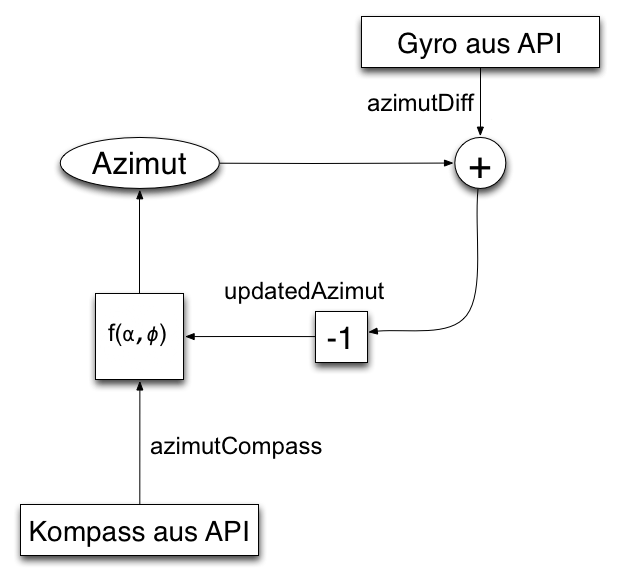
\includegraphics[scale=0.5]{figures/struktur}
\caption{Konzept Multisensordatenfusion}
\label{fig:struktur}
\end{figure}







\cleardoublepage

%%
%%%%%%%%%%%%%%%%%%%%%%%%%%%%%%%%%%%%%%%%%%%%%%%%%%%%%%%%%%%%%%%%%%%%
% Auswahl geeigneter Hardware
%%%%%%%%%%%%%%%%%%%%%%%%%%%%%%%%%%%%%%%%%%%%%%%%%%%%%%%%%%%%%%%%%%%%

\chapter{Plattform und Werkzeuge}
  \label{Plattform und Werkzeuge}
  
  \section{Plattform}
  
  \medskip
Bei der Suche nach einem passenden Gerät kamen mehere Kriterien zum Tragen. Es sollte wegen der Visualisierung größer als ein Smartphone sein, aber trotzdem portabler als ein herkömmliches Notebook. Es stand also fest, dass ein Tablet am besten geeignet ist für diese Art Anwendung. Desweiteren muss das Gerät mit den oben beschriebenen Sensoren, Accelerometer, Gyroskop und Kompass ausgestattet sein.

	\subsection{Überblick am Markt befindlicher Geräte}
Wirklich am Markt vertreten waren zum Zeitpunkt der Hardware-Entscheidung (Anfang 2011) nur das Apple iPad 1 und das Motorola Xoom. Das iPad war mit Accelerometer und Kompass ausgestattet, jedoch nicht mit einem Gyroskop. Das Motorola Xoom hatte alle drei IMUs verbaut. Android Version 3.0 Honeycomb erschien im Februar 2011 und war die erste Android-Version, die für Tablets ausgelegt war. \cite{ wiki:005} Allerdings war diese Version des Betriebssystems anfangs Berichten zufolge instabil.
	
	\subsection{Wahl iPad 2}
	Da das iPad 2 in den Startlöchern stand entschieden wir, unsere Entscheidung noch aufzuschieben. Am 11. März 2011 wurde es vorgestellt und die Ausstattung entsprach unseren Erwartungen, da es zusätzlich ein Gyroskop verbaut wurde. Zum Erscheinungszeitpunkt war Apple auch der Hersteller mit der meisten Erfahrung. Das iPad der ersten Generation war bereits ein Jahr auf dem Markt und hatte mit iOS ein ausgereiftes Betriebssystem. iOS wird auf dem Apple iPhone schon seit 2007 verwendet. Zudem war das iPad damals der unangefochtene Marktführer. Damit war auch gewährleistet, dass für eine eventuell entstehende App für Endanwender genügend potentielle Abnehmer bereit stünden.
	

\section{Werkzeuge}

\subsection{Frameworks}
Zur Erstellung von iOS-Programmen steht Entwicklern Cocoa Touch von Apple zur Verfügung. Cocoa Touch ist eine Sammlung von Frameworks, die Entwickler bei der Programmierung unterstützen sollen. Grob lassen sich drei Arten von Frameworks, die in Cocoa Touch enthalten sind, nennen:

\begin{itemize}
\item Funktionen der Hardware
\item Design-Elemente und Animationen
\item Verarbeitung von Daten
\end{itemize}

Cocoa Touch ist in Objective-C implementiert. Somit verwenden wir auch hauptsächlich Objective-C. \cite{apple:002}

Bei iOS sind für unsere Zwecke vor allem zwei Frameworks wichtig, die beide zum ersten Punkt der obigen Liste gehören. Core Location um den Kompass und Core Motion um das Gyroskop und das Accelerometer auszulesen.\\

\subsubsection{Core Motion}
Core Motion liefert Daten die, mit Bewegung zu tun haben. Das sind einerseits die rohen Daten aller drei Sensoren, die in Kapitel \ref{Konzept} beschrieben wurden. Andererseits stellt Core Motion aber auch bereits bereinigte Bewegungs-Daten zur Verfügung. Zum Beispiel lassen sich Beschleunigung und Gravitation getrennt auslesen. Core Motion nimmt auch bereits die Stabilisierung des Elevation-Werts des Gyroskop vor. Besonders interessant für unseren Anwendungsfall ist die Klasse \texttt{CMAttitude}. Sie beinhaltet die Orientierung des Geräts zum Zeitpunkt der Abfrage. \texttt{CMAttitude} stellt diese in allen drei in Kapitel \ref{Stand der Technik} beschriebenen Formen zur Verfügung.

\subsubsection{Core Location}
Core Location enthält alle Informationen, die zur Bestimmung der aktuellen Position und der Ausrichtung des Geräts nötig sind. Core Location ist auch in der Lage, aus einem Geocode die zugehörige Stadt zu ermitteln und anders herum. Für uns ist die Klasse \texttt{CMHeading} interessant. Sie stellt den aktuellen Kompass-Wert bereit.

\subsection{Unity}
Unity ist eine Spiele-Engine zur Entwicklung von Spielen für verschiedene Plattformen. Darunter sind PC-Betriebssyteme, mobile Betriebssyteme und Browser, aber auch herkömmliche Spiele-Konsolen. Unity ist neben der Unreal Engine eine der beliebtesten Spiele-Engines. In Unity kann man komplette 3D-Welten erstellen. Unity erlaubt den Export des Projekts in ein für die Zielplattform passendes Format. Im Falle von iOS wird ein Xcode Projekt erstellt. \cite{unity}

\subsection{Xcode}
Xcode ist die Entwicklungsumgebung für iOS-Anwendungen. In Xcode wird der Quellcode geschrieben und das Interface angeordnet. Mit Xcode kann die App, an der momentan gearbeitet wird, direkt auf ein angeschlossenes iOS-Gerät kompiliert werden. Am Ende wird mit Xcode auch die Datei zur Einreichung in den AppStore erstellt.
\cleardoublepage

%%
%%%%%%%%%%%%%%%%%%%%%%%%%%%%%%%%%%%%%%%%%%%%%%%%%%%%%%%%%%%%%%%%%%%%
% Umsetzung
%%%%%%%%%%%%%%%%%%%%%%%%%%%%%%%%%%%%%%%%%%%%%%%%%%%%%%%%%%%%%%%%%%%%

\chapter{Umsetzung}
  \label{Umsetzung}
  
\section{Unity-Integration}
Als Ausgangspunkt liegt eine voll funktionsfähige Navigations-App für Bibliotheken vor. Sie wurde komplett in Unity umgesetzt. Die Einbindung der Orientierungsberechnung kann nicht direkt in Unity vorgenommen werden, da in Unity nur ein eingeschränkter Zugang auf die Cocoa-Frameworks, die die APIs zum Zugriff auf die Hardware zur Verfügungs stellen, möglich ist. Darum wird die App ohne den Hardwarezugriff als Xcode Projekt exportiert. Dann muss in Xcode ein Plug-in programmiert werden, das als Schnittstelle zwischen selbst geschriebenem Objective-C-Code in Xcode, der die Hardware ausließt, und Unity dient. Dazu muss erst noch in Unity das Plug-in als Eingabe-Skript erstellt werden. Dieses Eingabe-Skript ist in C\# geschrieben.
~\\
\begin{lstlisting}[float=htb, caption=Plug-in in Unity, label=listing001]
[DllImport ("__Internal")]
private static extern CMQuaternion getDeviceMotion();
\end{lstlisting}
  
In Listing \ref{listing001}  wird also die externe Methode \texttt{getDeviceMotion()} aufgerufen. Das Plug-in erwartet den Datentyp \texttt{CMQuaternion}. Später wird ein Quaternion übergeben, also immer die aktuelle absolute Orientierung. \texttt{CMQuaternion} ist eigentlich ein Datentyp auf dem Core Motion Framework und somit Unity nicht bekannt. Darum muss erst noch ein \texttt{struct} mit der Bezeichung \texttt{CMQuaternion} definiert werden (Listing \ref{listing002}).
~\\
\begin{lstlisting}[float=htb, caption=Struct \texttt{CMQuaternion} in C\#, label=listing002]
public struct CMQuaternion {
	public double x, y, z, w;
}
\end{lstlisting}

Alles weitere erfolgt jetzt direkt in Xcode. In Xcode wird eine \texttt{*.mm}-Datei angelegt zusammen mit der zugehörigen \texttt{*.h}-Datei. In der \texttt{*.mm}-Datei erfolgt die ganze Implementierung. Damit in der bestehenden App überhaupt Daten, die hier berechnet werden ankommen, muss als erstes die \texttt{getDeviceMotion()}-Methode implementiert werden:
~\\
\begin{lstlisting}[float=htb, caption=Methode \texttt{getDeviceMotion}, label=listing003]
static GyroscopeData* delegateObject = nil;

extern "C" {

	CMQuaternion getDeviceMotion () {

		if (delegateObject == nil) {
			delegateObject = [[GyroscopeData alloc] init];
		}
		
		return [delegateObject getOrientation];(*@\label{line001}@*)
	}    
}
\end{lstlisting}

Allerdings muss in dieser \texttt{extern  C }-Umgebung in C geschrieben werden. In C sind aber die API-Aufrufe nicht oder nur sehr umständlich möglich. Darum wird in Zeile \ref{line001} in Listing \ref{listing003} eine weitere Methode \texttt{getOrientation} aufgerufen. 
~\\
\begin{lstlisting}[float=htb, caption=Methode \texttt{getOrientation}, label=listing004]
- (CMQuaternion)getOrientation {
	...
	...
}
\end{lstlisting}

Diese Methode (Listing \ref{listing004})  enthält den eigentlichen Objective-C-Quellcode. In ihr können alle API-Aufrufe problemlos ausgeführt werden. 

In Abbildung \ref{fig:unity-integration} wird der Zusammengang der Methoden und Dateien nochmal schematisch dargestellt.

\cite{unity}

\begin{figure}[htb]
\centering
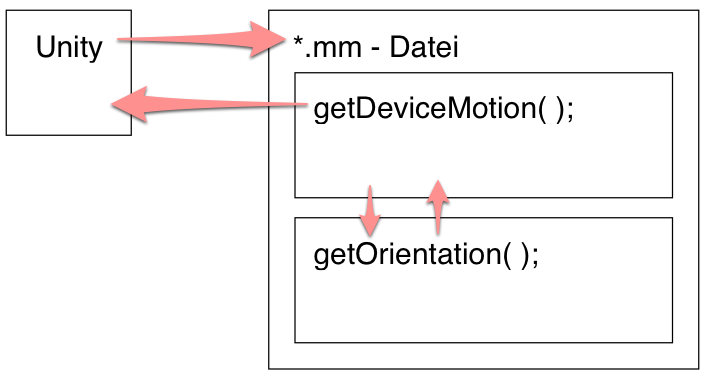
\includegraphics[scale=0.5]{figures/unity-integration}
\caption{Unity-Integration}
\label{fig:unity-integration}
\end{figure}
  
\section{Vorbereitung der nötigen Daten}
Um die Multidatenfusion durchführen zu können, müssen erst alle nötigen Daten ausgelesen werden. Dazu müssen \texttt{CMMotionManager}- und \texttt{CLLocationManager}-Objekte initialisert werden.  \cite{book001} \cite{book002} 
~\\
\begin{lstlisting}[float=htb, caption=\texttt{locationManager} und \texttt{motionManager} initialisieren \cite{apple:003}, label=listing005]
// Set up locationManager
if (locationManager == nil) {
	locationManager=[[CLLocationManager alloc] init];
	locationManager.desiredAccuracy = kCLLocationAccuracyBest;(*@\label{line002}@*)
}
    
// Set up motionManager    
if (motionManager == nil) {
	motionManager = [[CMMotionManager alloc] init];
	motionManager.deviceMotionUpdateInterval = 1.0/60.0;(*@\label{line003}@*)
}
\end{lstlisting}

In Zeile \ref{line002} in Listing \ref{listing005} wird die Genauigkeit des \texttt{CLLocationManager}-Objekts und in Zeile \ref{line003} die Update-Frequenz des \texttt{CMMotionManager}-Objekts eingestellt. Der Kompass-Wert, der aus dem \texttt{CLLocationManager}-Objekt ausgelesen wurde, muss sehr genau sein.

Das Auslesen des Kompass-Werts findet eventgesteuert statt. Ein neuer Wert wird nur dann ausgelesen, wenn er sich vom alten Wert unterscheidet. Dazu wird die minimale Winkeländerung auf $1^o$ festgesetzt.
~\\
\begin{lstlisting}[float=htb, caption=\texttt{locationManager} starten \cite{apple:003}, label=listing006]
// Start listening to events from locationManager
if ([CLLocationManager headingAvailable]) {
	locationManager.headingFilter = 1;
	[locationManager startUpdatingHeading];(*@\label{line004}@*)
}
\end{lstlisting}

Mit dem Aufrufen der Methode \texttt{startUpdatingHeading} in Zeile \ref{line004} in Listing \ref{listing006} wird hier auch gleichzeitig das eventgesteuerte Abfragen des Kompass-Werts gestartet.

Die Methode, die auf die Kompass-Änderungen (Listing \ref{listing007}) hört, liest den Kompass-Wert aus und stellt ihn in einer globalen Variable zur Verfügung.
~\\
\begin{lstlisting}[float=htb, caption=Azimut ermittelt durch Kompass, label=listing007]
- (void)locationManager:(CLLocationManager *)manager didUpdateHeading:(CLHeading *)newHeading {
	// Get new heading
	mHeading = newHeading.magneticHeading;    
    
	//location specific offset depending on the 3D model
	locationOffset = 90;
	mHeading += locationOffset;
    
	if (mHeading > 360) {
		mHeading -= 360;
	}
	else if (mHeading < 0) {
		mHeading += 360;
	}
}
\end{lstlisting}

Es kann vorkommen, dass in dem 3D-Modell des Raums nicht an der selben Stelle Norden ist wie in der Realität an diesem Ort. Darum muss, wenn dieser Fall auftritt, ein Offset zu dem ausgelesenen Wert addiert werden. Das Resultat kann ein Wert sein, der entweder größer als $360^o$ oder kleiner als $0^o$ ist. Der Wert muss dann normalisiert werden indem $360^o$ subtrahiert oder addiert werden. Das Ergebnis ist der Azimut-Wert, ermittelt durch den Kompass.

Die Azimut-Änderung, ermittelt durch das Gyroskop und die Elevation, liefert das \texttt{CMMotionManager}-Objekt.
~\\
\begin{lstlisting}[float=htb, caption=Bewegungsdaten auslesen \cite{apple:003}, label=listing008]
if(motionManager.isDeviceMotionAvailable) {
        
	// Listen to events from the motionManager
	motionHandler = ^ (CMDeviceMotion *motion, NSError *error) {
	
	CMAttitude *currentAttitude = motion.attitude;(*@\label{line005}@*)
	.
	.
	.
}
\end{lstlisting}

Im \texttt{CMDeviceMotion}-Objekt werden Messungen des Accelerometers und des Gyroskops zusammengefasst. Der \texttt{motionHandler} wird immer dann aufgerufen, wenn es Bewegungs-Daten des Geräts zu verarbeiten gibt. Hier ist das alle 1/60 Sekunden der Fall, weil das bei der Initialisierung des \texttt{CMMotionManager}-Objekts so festgelegt wurde.

Das Auslesen der eigentlichen Orientierungsdaten erfolgt in Zeile \ref{line005} von Listing \ref{listing008}. Wobei in diesem \texttt{CMAttitude}-Objekt alle drei Beschreibungs-Möglichkeiten, Euler-Winkel, Rotationsmatrix und Quaternion, zusammengefasst sind.
~\\
\begin{lstlisting}[float=htb, caption=Azimut-Änderung berechnen, label=listing009]
quaternion = currentAttitude.quaternion;

if (oldQuaternion.w != 0 || oldQuaternion.x != 0 || oldQuaternion.y != 0 || oldQuaternion.z != 0){
	diffQuaternion = [self multiplyQuaternions:[self inverseQuaternion:oldQuaternion] :quaternion];
	diffQuaternion = [self normalizeQuaternion:diffQuaternion];
}            
oldQuaternion = quaternion;
\end{lstlisting}

Die Orientierung wird als Queternion ausgelesen und die Differenz zur letzten Orientierung gespeichert. Dies wird erreicht indem der inverse Quaternion des alten Werts mit dem Quaternion des neuen Werts multipliziert wird. Danach muss das Ergebnis noch normalisiert werden. Das geschieht in Listing \ref{listing009} mit Hilfe der vier Methoden \texttt{quaternionMagnitude} (Listing \ref{listing010}), \texttt{inverseQuaternion} (Listing \ref{listing011}), \texttt{multiplyQuaternions} (Listing \ref{listing012}) und \texttt{normalizeQuaternion} (Listing \ref{listing013}).
~\\
\begin{lstlisting}[float=htb, caption=Methode \texttt{quaternionMagnitude}, label=listing010]
- (float) quaternionMagnitude:(CMQuaternion)inputQuaternion {
	float magnitude = sqrt(inputQuaternion.w*inputQuaternion.w + inputQuaternion.x*inputQuaternion.x + inputQuaternion.y*inputQuaternion.y + inputQuaternion.z*inputQuaternion.z);
	
	return magnitude;
}
\end{lstlisting}


\begin{lstlisting}[float=htb, caption=Methode \texttt{inverseQuaternion}, label=listing011]
- (CMQuaternion) inverseQuaternion:(CMQuaternion)inputQuaternion {
	float magnitude = [self quaternionMagnitude:inputQuaternion];
	
	quaternion.w = inputQuaternion.w/magnitude;
	quaternion.x = -inputQuaternion.x/magnitude;
	quaternion.y = -inputQuaternion.y/magnitude;
	quaternion.z = -inputQuaternion.z/magnitude;
	
	return quaternion;
}
\end{lstlisting}

\begin{lstlisting}[float=htb, caption=Methode \texttt{multiplyQuaternions}, label=listing012]
- (CMQuaternion) multiplyQuaternions:(CMQuaternion)quaternionA:(CMQuaternion)quaternionB {
	quaternion.w = quaternionA.w*quaternionB.w - quaternionA.x*quaternionB.x - quaternionA.y*quaternionB.y - quaternionA.z*quaternionB.z;
	quaternion.x = quaternionA.w*quaternionB.x + quaternionA.x*quaternionB.w - quaternionA.y*quaternionB.z + quaternionA.z*quaternionB.y;
	quaternion.y = quaternionA.w*quaternionB.y + quaternionA.x*quaternionB.z + quaternionA.y*quaternionB.w - quaternionA.z*quaternionB.x;
	quaternion.z = quaternionA.w*quaternionB.z - quaternionA.x*quaternionB.y + quaternionA.y*quaternionB.x + quaternionA.z*quaternionB.w;

	return quaternion;
}
\end{lstlisting}

\begin{lstlisting}[float=htb, caption=Methode \texttt{normalizeQuaternion}, label=listing013]
- (CMQuaternion) normalizeQuaternion:(CMQuaternion)inputQuaternion {
	float magnitude = [self quaternionMagnitude:inputQuaternion];
	
	quaternion.w = inputQuaternion.w / magnitude;
	quaternion.x = inputQuaternion.x / magnitude;
	quaternion.y = inputQuaternion.y / magnitude;
	quaternion.z = inputQuaternion.z / magnitude;
	
	return quaternion;
}
\end{lstlisting}

Die interessanten Werte, Azimut und Elevation, werden aus dem Quaternion in Grad berechnet. Die Methoden \texttt{azimutFromQuaternion} (Listing \ref{listing014}) und \texttt{elevationFromQuaternion}  (Listing \ref{listing015}) berechnen den entsprechenden Winkel in Radian.
~\\
\begin{lstlisting}[float=htb, caption=Azimut-Wert aus Quaternion berechnen, label=listing014]
- (float) azimutFromQuaternion:(CMQuaternion)quaternion {
	float azimut = atan2(2*(quaternion.w*quaternion.z+quaternion.x*quaternion.y), 1 - 2*(quaternion.y*quaternion.y+quaternion.z*quaternion.z));
	return azimut;
}

azimutDiff = RADIANS_TO_DEGREES([self azimutFromQuaternion:diffQuaternion]);
\end{lstlisting}

\begin{lstlisting}[float=htb, float=htb, caption=Elevation-Wert aus Quaternion berechnen, label=listing015]
- (float) elevationFromQuaternion:(CMQuaternion)quaternion {
	float elevation = atan2(2*(quaternion.w * quaternion.x + quaternion.y * quaternion.z), 1-2 * (quaternion.x * quaternion.x + quaternion.y * quaternion.y));
	return elevation;
} 

elevation = -[self elevationFromQuaternion:quaternion];
elevation += M_PI/2;
elevation = RADIANS_TO_DEGREES(elevation);
\end{lstlisting}

Bei der Elevation muss noch eine Korrektur von $90^o$ vorgenommen werden. Denn wenn man das iPad mit dem Display nach oben um $90^o$ neigt, sodass das Display zum Betrachter zeigt, befindet sich standardmäßig genau in dieser Position der Sprung von $0^o$ auf $360^o$. Um eventuellen Problemen mit dieser Tatsache aus dem Weg zu gehen, wird der Sprung um $90^o$ nach oben verschoben. Dann tritt er nur auf wenn der Betrachter das iPad direkt an die Decke hält. \cite{paper:001} \cite{mathworks}

\section{Multisensordatenfusion}
Nur der Azimut-Wert muss noch selbst berechnet werden. Das Core Motion-Framework liefert bereits einen mit dem Accelerometer stabilisierten Elevation-Wert. Darum weist der in Listing \ref{listing015} berechnete Elevation-Wert keinen bemerkbaren Drift mehr auf.

Nun kann die Formel aus Kapitel \ref{formula001} umgesetzt werden.
~\\
\begin{lstlisting}[float=htb, caption=Eigentliche Datenfusion, label=listing016]
updatedAzimut = updatedAzimut - azimutDiff;(*@\label{line006}@*)

float alpha = 19.0;
float phi = 1.0;

//fusionate gyro estimated heading with new magneticHeading
updatedAzimut = (alpha* updatedAzimut + phi*heading)/(alpha+phi);(*@\label{line007}@*)         
\end{lstlisting}

In Zeile \ref{line006} aus Listing \ref{listing016} wird die Azimut-Änderung auf den vorherigen Azimut-Wert angewendet. Zeile \ref{line007} ist die genaue Umsetzung der Formel aus Kapitel \ref{formula001}. \texttt{updatedAzimut} ist der zur Drehung verwendete Azimut-Wert korrigiert um die Drehung seit dem letzten Wert. \texttt{heading} ist der durch den Kompass bestimmte Azimut-Wert. Mit den beiden Steuerungsvariablen \texttt{alpha} und \texttt{phi} wird gesteuert welche Anteile die jeweiligen Komponenten der Fusion haben.
~\\
\begin{lstlisting}[float=htb, caption=Generierung des Endergebnisses, label=listing017]
rotation = [self createFromAxisAngle:0 :elevation :DEGREES_TO_RADIANS(updatedAzimut)];
return rotation;
\end{lstlisting}
~\\
\begin{lstlisting}[float=htb, caption=Generierung eines Quaternions aus Euler-Winkeln, label=listing018]
- (CMQuaternion) createFromAxisAngle:(double)roll:(double)pitch:(double)yaw {
	CMQuaternion quaternion;
	
	float num9 = roll * 0.5f;
	float num6 = (float) sin((double) num9);
	float num5 = (float) cos((double) num9);
	float num8 = pitch * 0.5f;
	float num4 = (float) sin((double) num8);
	float num3 = (float) cos((double) num8);
	float num7 = yaw * 0.5f;
	float num2 = (float) sin((double) num7);
	float num = (float) cos((double) num7);
	quaternion.w = ((num * num3) * num5) + ((num2 * num4) * num6);
	quaternion.x = ((num * num4) * num5) + ((num2 * num3) * num6);
	quaternion.y = ((num2 * num3) * num5) - ((num * num4) * num6);
	quaternion.z = ((num * num3) * num6) - ((num2 * num4) * num5);
	
	return quaternion;
}
\end{lstlisting}

Mit Listing \ref{listing017} wird das Ergebnis zusammengefasst. Aus \texttt{elevation} und \texttt{updatedAzimut} wird mittels der Methode \texttt{createFromAxisAngle} (Listing \ref{listing018}) der Quaternion \texttt{rotation} generiert. Er ist die Rückgabe dieser Funktion und wird vom Plug-in in Unity erwartet.

\section{Test-App}
\begin{figure}[htb]
\centering
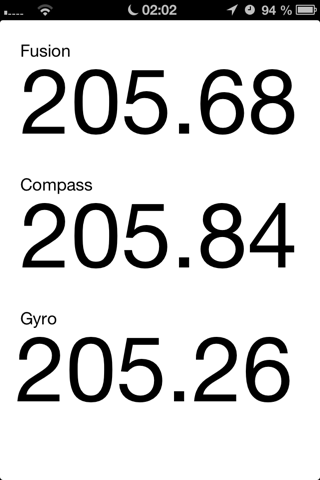
\includegraphics[scale=0.6]{figures/testapp}
\caption{Test-App}
\label{fig:testapp001}
\end{figure}
Um die folgenden Messungen und Grafiken für den Ergebnis-Teil zu ermitteln, wurde eine eigene Test-App erstellt. Diese teilt sich mit der Navigations-App den selben Quellcode bezüglich der Orientierung. Allerdings besteht die Test-App nur aus dem Code, der für die Orientierungsberechnungen wichtig ist, erweitert um eine Funktion, die die berechneten Werte in eine SQLite-Datenbank schreibt. Zusätzlich zeigt die App die drei relevanten Werte auch auf dem Display zur Kontrolle an. Immer wenn die App gestartet bzw. aufgerufen wird, wird eine neue Messung gestartet. Falls eine SQLite-Datei von einer vorherigen Messung noch vorhanden ist, wir diese überschrieben. Das Beenden der App durch Drücken des Home-Buttons beendet auch die Aufzeichnung der Werte. Die SQLite-Datei kann nun bequem aus iTunes heraus auf einem Computer zur Weiterverabreitung gespeichert werden.


\cleardoublepage

%%
%%%%%%%%%%%%%%%%%%%%%%%%%%%%%%%%%%%%%%%%%%%%%%%%%%%%%%%%%%%%%%%%%%%%
% Ergebnis
%%%%%%%%%%%%%%%%%%%%%%%%%%%%%%%%%%%%%%%%%%%%%%%%%%%%%%%%%%%%%%%%%%%%

\chapter{Ergebnis}
  \label{Ergebnis}


Eine funktionierende Orientierung lässt sich bereits mit Kompass und dem Pitch-Wert den das Gyroskop liefert realisieren.

\cleardoublepage

%%
\chapter{Ausblick}
  \label{Ausblick}
Die naheliegendste Weiterentwicklungsmöglichkeit ist mit Sicherheit Augmented Reality. Das bedeutet, man verzichtet auf das vollständige 3D-Modell um die Bibliothek nachzubilden und nutzt stattdessen die Kamera des Geräts. Auf das Kamera-Bild kann man dann die Navigationspfeile, Markierungen und sonstige Informationen einzeichnen. Augmented Reality hat aber den Nachteil, dass die Genauigkeit nochmal deutlich höher sein muss, als wenn man mit einem 3D-Modell arbeitet. Denn Ungenauigkeiten fallen viel stärker auf, da der abgebildete Raum immer der reale Raum ist. Beim 3D-Modell ist es weniger auffällig wenn die zugrundeliegenden Berechnungen nicht ganz korrekt sind, weil man zwischen Navigation und Realität noch das 3D-Modell als Puffer hat. Das 3D-Modell ist dennoch nach wie vor nötig. Es wird wie bisher auch gebraucht, um die Position der Bücher in den Regalen zu vermerken und um die Wege zu berechnen. Es ist nur unsichtbar, das heißt es fällt auch der Wartungsaufwand bei sich ändernden Regalinhalten weg.

Die erforderliche Genauigkeit ist mit der hier angewendet Sensorfusion noch nicht am Ende ihrer Möglichkeiten. Der Kalman-Filter ist in der Lage, die Ungenauigkeit der Sensoren weiter herauszurechnen. Da die Genauigkeit der Position auch eines der größten Probleme bei der Berechnung der Orientierung ist, würde der Kalman-Filter auch bei der Positionsbestimmung hilfreich sein. Aufgrund der IMUs könnte mit Hilfe des Kalman-Filters auch eine Position bestimmt werden. Diese kann man mit den RSSI-Werten der Bluetooth-Sender und dem Partikelfilter fusionieren und so die Position weiter verbessern. Diese Berechnungen sind allerdings sehr schwierig, da, aufgrund der Geräte-Größe, die Sensoren immer merkbare Fehler produzieren werden. Es muss das richtige Mischungsverhältnis der verschiedenen Sensoren und Verfahren gefunden werden. Das beste Mischungsverhältnis kann aber zusätzlich auch von der aktuellen Art der Bewegung abhängig sein. Dies stellt eine zusätzliche Schwierigkeit dar. Die Entwicklung eines wirklich guten Kalman-Filters für Orientierungs- und Positionsdaten setzt eine große Menge theoretisches Vorwissen und vor allem Test-Zeit voraus. Dies wäre im Rahmen einer Studienarbeit leider nicht möglich gewesen.

Wenn das Kamerabild sowieso schon für Augmented Reality verwendet wird, könnte man die Positionsgenauigkeit zusätzlich durch Bilderkennung unterstützen. Ähnlich wie bei modernen Autos, die anhand der Fahrbahnmarkierung und der Leitplanken versuchen die Spur zu halten, könnten die Bilddaten mit einem internen 3D-Modell abgeglichen werden. So könnte geprüft werden, ob man sich wirklich gerade an der berechneten Stelle befindet. Wenn diese Überprüfung ständig stattfinden kann, kann sie sogar laufend in die Positions- und Orientierungsberechnung einfließen. Allerdings nur wenn es Sinn macht. Böden, Wände oder auch Regalansichten sehen oft sehr ähnlich aus, sodass keine verlässliche Aussage darüber getroffen werden kann wo man sich befindet.
Das Problem bei der Bildverarbeitung in Echtzeit ist der große Rechenaufwand. Es müsste ca. 20 mal in der Sekunde ein komplettes Bild analysiert werden. Das ist eine sehr große Herausforderung für die mobilen Prozessoren. Dennoch könnte auch eine weniger häufige Bildanalyse hilfreich sein. Es könnte dazu dienen die anderen Berechnungen zu verifizieren.

Um die Stabilität der Orientierungsberechnung weiter zu verbessern, könnte eine Magnetfeld-Störungs-Erkennung realisiert werden. Dazu müsste die Orientierung des Kompasses beobachtet werden und wenn eine, verglichen mit den Orientierungs-Daten der anderen Sensoren, unnatürliche Bewegung auftritt, eine Art Reaktions-Schwellenwert greifen. Das heißt, wenn der Kompass eine Drehung feststellt, aber das Gyroskop völlig ruhig bleibt, ist anzunehmen, dass eine Störung durch ein Magnetfeld vorliegt. Die genaue Umsetzung wird aber ebenfalls schwierig sein, denn die Fehler beider Sensoren dürfen nicht als unterschiedliche Drehung erkannt werden. Apple hat dieses Problem bereits selbst erkannt. Die API liefert auch schon deutlich stabilere Werte als zu Anfang.

Nützlich für die Navigation in Bibliotheken ansich könnte die NFC-Technik werden. Diese kleinen Chips sind schon heute keine Seltenheit in Bibliotheks-Büchern. Zum einen können sie zur Orientierung dienen. Über die gefundenen Bücher in der Umgebung kann der Standort relativ genau berechnet werden und als weiterer Fusionsinput für die Positionsbestimmung dienen. Zum anderen kann man mit NFC auch eine automatische Bibliotheks-Inventur durch normale Benutzer realisieren. Die App kann beim normalen Gang durch die Bibliothek die Bücher in der Umgebung erkennen und zumindest ihre ungefähre, auf ca. drei Meter genaue, Position bestimmen. Diese würde auf dem Bibliotheks-Server mit der korrekten Position abgeglichen. Wenn der Unterschied zu groß ist würden die Mitarbeiter der Bibliothek informiert. In der Zwischenzeit wird der neue, aber falsche Standort auf dem Server als aktuelle Position des Buches gespeichert, damit auch andere Bibliotheks-Besucher das Buch, trotz falscher Position, mit der Navigations-App finden können. Diese Technik ist bei wenigen Geräten bereits eingebaut. Allgemein steht sie aber, wenn man die Patent-Anmeldungen der Hersteller der letzten Jahre verfolgt, auf jeden Fall in den Startlöchern. \cite{wiki:006}

Um den Nutzerkreis einer solchen App zu vergrößern ist es auch empfehlenswert, die App für andere Geräte und Systeme neben iOS, wie zum Beispiel Android und Windows Phone,  zu entwickeln. Das Grundgerüst der App sollte dank Unity leicht auf andere Plattformen portierbar sein. Nur die API-Aufrufe müssen an das jeweilige System angepasst werden.
\cleardoublepage


%%%%%%%%%%%%%%%%%%%%%%%%%%%%%%%%%%%%%%%%%%%%%%%%%%%%%%%%%%%%%%%%%%%%%%%%%%%%%
%%% Bibliographie
%%%%%%%%%%%%%%%%%%%%%%%%%%%%%%%%%%%%%%%%%%%%%%%%%%%%%%%%%%%%%%%%%%%%%%%%%%%%%

\addcontentsline{toc}{chapter}{Literaturverzeichnis}

\bibliographystyle{alpha}
\bibliography{mylit}
%% Obige Anweisung legt fest, dass BibTeX-Datei `mylit.bib' verwendet
%% wird. Hier koennen mehrere Dateinamen mit Kommata getrennt aufgelistet
%% werden.

\cleardoublepage

\end{document}

